\section{High Band Improvement}
From the S-parameter measurements of both the triangle feed antenna and the minimized monopole antenna it is clear that both antennas are experiencing problems in the high band.
The problem occured when going from the WiSpy board without the chip to the final board with the communication PCB, battery and the WiSpy chip. It seemed that, despite different antenna structures, the antennas were detuned when measured on the final WiSpy board.
The first approach was to counteract the high band problem by creating another resonance at an even higher frequency than required. The minimized monopole was modified to be a four arm monopole with an extra resonance at approx. \SI{2.7}{GHz} for both the top and side antenna. The technical drawing of the modified monopole can be seen on Figure \ref{fig:sparam_5mm_highband} together with a Table \ref{fig:sparam_5mm_highband}of the component values used in the simulation.
Furthermore to find the course of the problem an investigation was made to wheater the detuning was caused by the communication PCB, battery or the WiSpy chip. 

\begin{figure}[htbp]
    \begin{subfigure}[b]{0.49\linewidth}
        \centering
        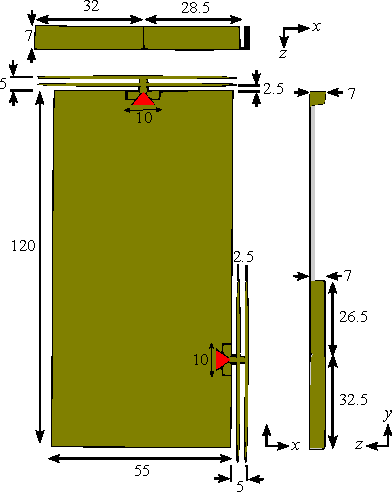
\includegraphics{img/tech_sol/monopole/highband/3d_drawing}
        \caption{Technical drawing.}
        \label{fig:ant1technical_highband}
    \end{subfigure}
    \hfill
    \begin{subfigure}[b]{0.49\linewidth}
        \centering
        \includegraphics{img/tech_sol/schematic_tuning_1}\\[1cm]
\footnotesize
        \begin{tabular}{|l|l|l|l|}
            \hline
            & $C_1$ & $L_1$ & $C_2$ \\
            \hline
            Top antenna & \SI{3.02}{pF} & \SI{7.99}{nH} & $[0.3,2.9]\,$pF\\
            Side antenna & \SI{1.81}{pF} & \SI{5.27}{nH} & $[0.3,2.9]\,$pF\\
            \hline
        \end{tabular}
        \caption{Tuning/matching circuit.}
        \label{fig:ant1_tuning_highband}
    \end{subfigure}
    \caption{Technical drawing and tuning circuit for the antenna.  The matching circuit is applied for both the top and the side antenna.}
    \label{fig:sparam_5mm_highband}
\end{figure}

\FloatBarrier
\subsection{Modified Monopole Simulation}

The S-parameter sweep can be seen on Figure \ref{fig:sparam_mono_modi_sim}

% Sweeping S-parameters
\begin{figure}[htbp]
   \begin{subfigure}[b]{0.49\linewidth}
        \centering
        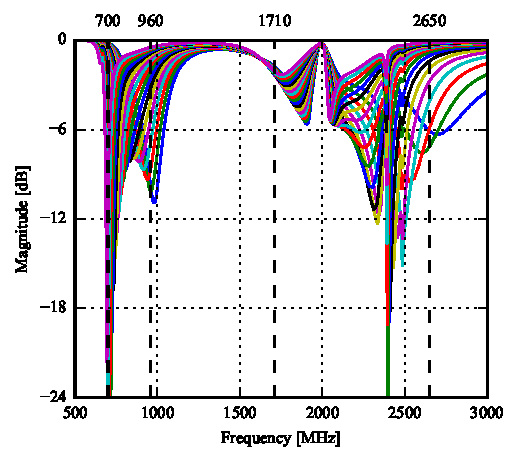
\includegraphics{img/tech_sol/monopole/highband/sim/s11.pdf}
        \caption{$S_{11}$, sweeping $C_1$ and fixing $C_2$.}
   \end{subfigure}
    \hfill
    \begin{subfigure}[b]{0.49\linewidth}
        \centering
        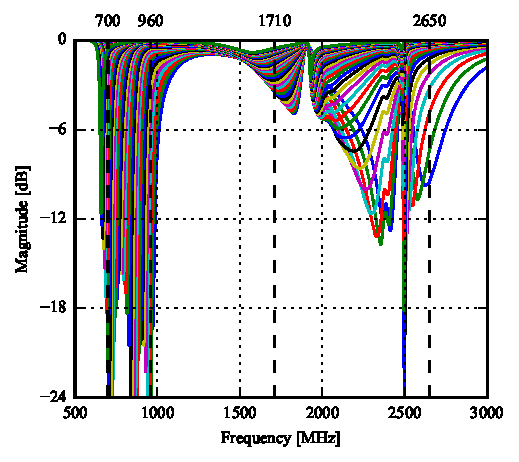
\includegraphics{img/tech_sol/monopole/highband/sim/s22.pdf}
        \caption{$S_{22}$, sweeping $C_2$ and fixing $C_1$.}
    \end{subfigure}
~
    \begin{subfigure}[b]{0.49\linewidth}
        \centering
        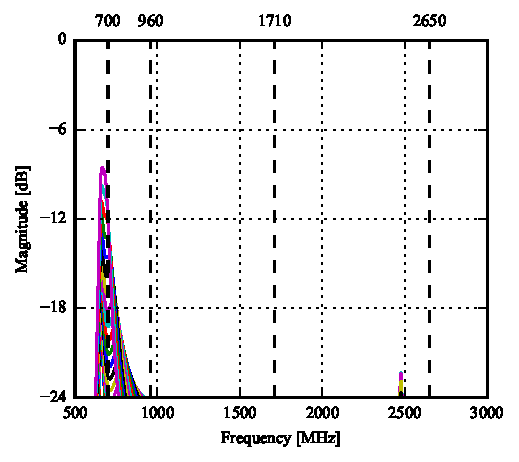
\includegraphics{img/tech_sol/monopole/highband/sim/s11_s21.pdf}
        \caption{$S_{21}$, sweeping $C_1$ and fixing $C_2$.}
    \end{subfigure}
    \hfill
    \begin{subfigure}[b]{0.49\linewidth}
        \centering
        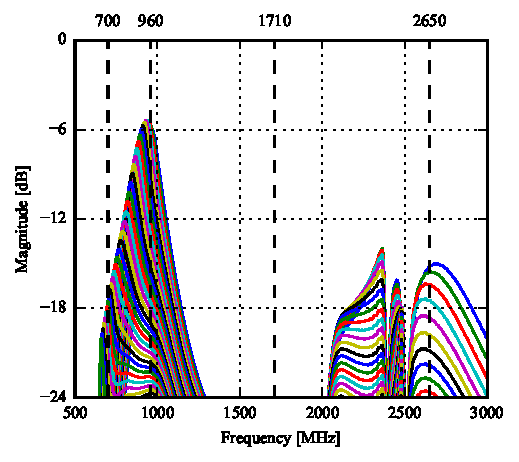
\includegraphics{img/tech_sol/monopole/highband/sim/s22_s21.pdf}
        \caption{$S_{21}$, sweeping $C_2$ and fixing $C_1$.}
    \end{subfigure}
    \caption{S-parameter sweep in free space for tuning the shunt capacitor of each antenna, $C_1$ and $C_2$ for port 1 and 2, respectively. Port 1 is the top antenna and port 2 is the side antenna.}
    \label{fig:sparam_mono_modi_sim}
\end{figure}

\FloatBarrier
\subsection{Modified Monopole Measurements}

\begin{figure}[htbp]
        \centering
        \begin{tabular}{m{3in}m{3in}}
            \centering
            \includegraphics{img/tech_sol/schematic_tuning_1}&
            \centering
            \footnotesize
            \begin{tabular}{|l|l|l|l|}
                \hline
                & $C_1$ & $L_1$ & $C_2$ \\
                \hline
              Top antenna & \SI{3.9}{pF} & \SI{2.2}{nH} & \SI{0.6}{pF} \\
              Side antenna & \SI{4}{pF} & \SI{1}{nH} & \SI{1.2}{pF} \\
                \hline
            \end{tabular}
        \end{tabular}
    \caption{Matching circuit for the minimized monopole prototype. These are the component values where the bandwidth is found to be the largest.}
    \label{fig:mono_matching_modi_meas}
\end{figure}

\begin{figure}[htbp]
   \begin{subfigure}[b]{0.49\linewidth}
        \centering
        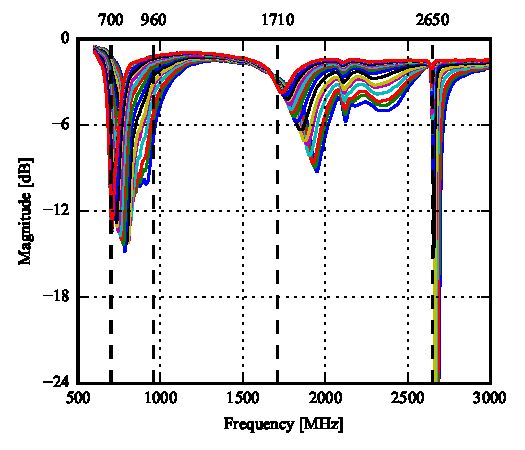
\includegraphics{img/tech_sol/monopole/highband/meas/tuner/S11.pdf}
        \caption{$S_{11}$, sweeping $C_1$ and fixing $C_2$.}
    \end{subfigure}
    \hfill
    \begin{subfigure}[b]{0.49\linewidth}
        \centering
        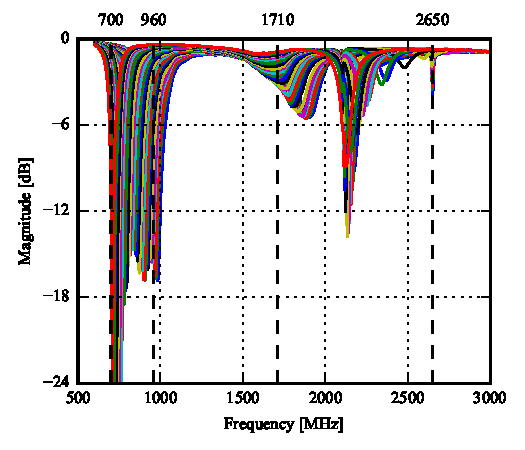
\includegraphics{img/tech_sol/monopole/highband/meas/tuner/S22.pdf}
        \caption{$S_{22}$, sweeping $C_2$ and fixing $C_1$.}
    \end{subfigure}
~
    \begin{subfigure}[b]{0.49\linewidth}
        \centering
        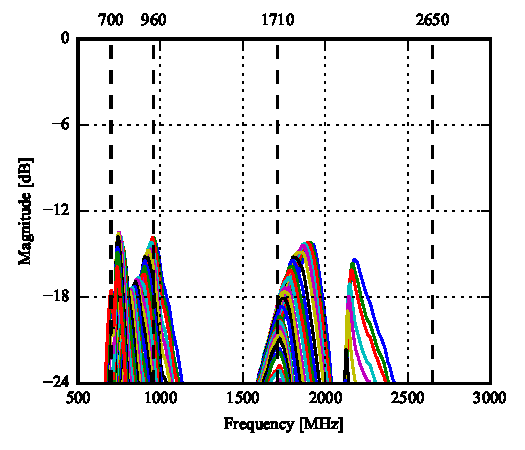
\includegraphics{img/tech_sol/monopole/highband/meas/tuner/S21.pdf}
        \caption{$S_{21}$, sweeping $C_1$ and fixing $C_2$.}
    \end{subfigure}
    \hfill
    \begin{subfigure}[b]{0.49\linewidth}
        \centering
        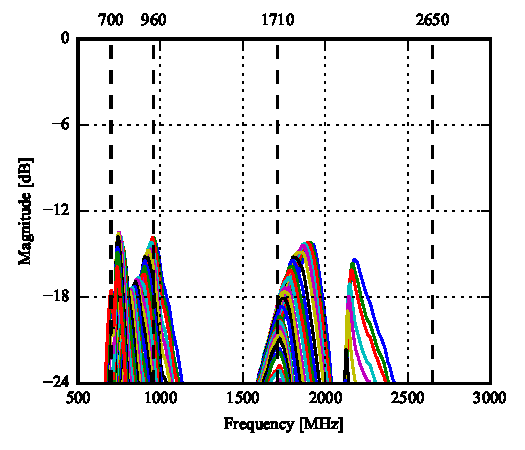
\includegraphics{img/tech_sol/monopole/highband/meas/tuner/S21.pdf}
        \caption{$S_{21}$, sweeping $C_2$ and fixing $C_1$.}
    \end{subfigure}
    \caption{S-parameter sweep in free space for tuning the shunt capacitor of each antenna, $C_1$ and $C_2$ for port 1 and 2, respectively. Port 1 is the top antenna and port 2 is the side antenna.}
    \label{fig:sparam_mono_modi_meas}
\end{figure}

\FloatBarrier
\subsection{Detuning Investigation}

\begin{figure}[htbp]
   \begin{subfigure}[t]{0.49\linewidth}
        \centering
        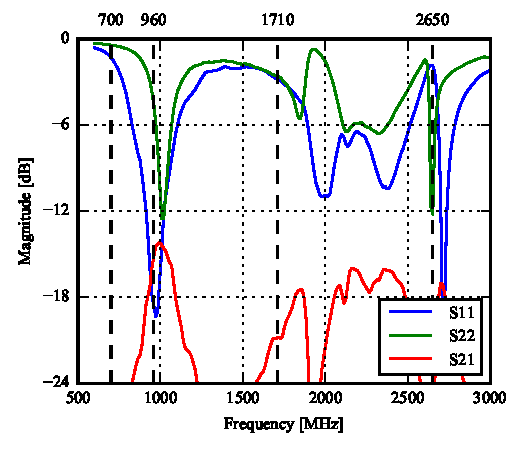
\includegraphics{img/tech_sol/monopole/highband/meas/no_tuner/sparams_best_match.pdf}
        \caption{S-parameters for the modified monopole antenna without the tuner.}
        \label{fig:sparams_notuner_mono_modi_meas}
    \end{subfigure}
    \hfill
    \begin{subfigure}[t]{0.49\linewidth}
        \centering
        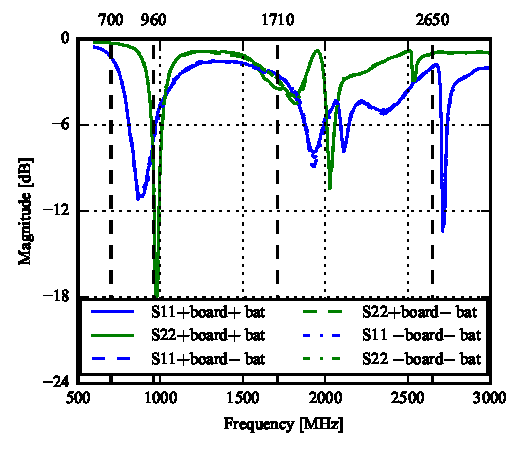
\includegraphics{img/tech_sol/monopole/highband/meas/tuner_comparison/sparam_comparison}
        \caption{S-parameter comparison of the WiSpy board with and without the battery and communication PCB.}
        \label{fig:sparams_tuner_mono_modi_meas}
    \end{subfigure}
    \caption{S-parameter comparison of WiSpy PCB's}
    \label{fig:sparams_comp_mono_modi_meas}
\end{figure}